\chapter{
تصویر تصادفی پایدار
}

روش تصویر تصادفی پایدار
\LTRfootnote{Stable Random Projections}
\cite{litez116, litez166, litez19, litez99, litez96, litez104}
یک روش پرکاربرد در داده‌کاوی و یادگیری ماشین است. با این روش به طور کار 
$l_\alpha (0 < \alpha \leq 2)$
فاصله در داده‌های حجیم (برای مثال: وب یا جریان‌های داده‌ی حجیم) محاسبه می‌شود. در این روش حافظه‌ی کمی استفاده شده و فقط یک بار پایش داده‌ها کافی است. 

\begin{figure}[h]
\centering
\begin{latin}
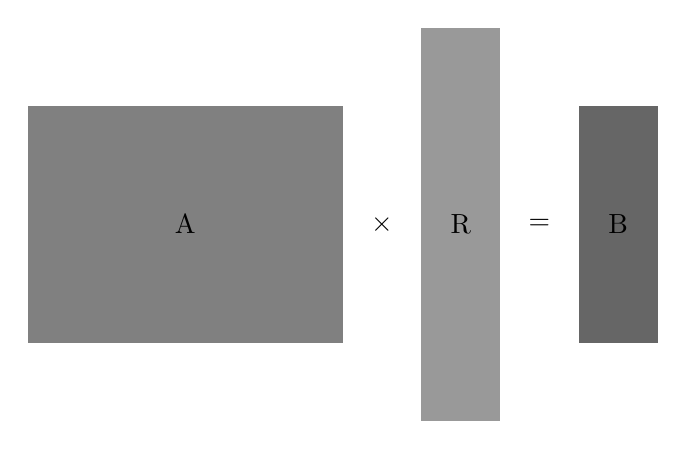
\begin{tikzpicture}
\fill[black!50!white] (0,1) rectangle (4,4);
\node at (2,2.5) [rectangle,preaction={fill=black!50},font={A}] {};
\node at (4.5,2.5) [rectangle,preaction={fill=black!0},font={$\times$}] {};
\fill[black!40!white] (5,0) rectangle (6,5);
\node at (5.5,2.5) [rectangle,preaction={fill=black!40},font={R}] {};
\node at (6.5,2.5) [rectangle,preaction={fill=black!0},font={=}] {};
\fill[black!60!white] (7,1) rectangle (8,4);
\node at (7.5,2.5) [rectangle,preaction={fill=black!60},font={B}] {};
\end{tikzpicture}
\end{latin}
\caption{
روش تصویر تصافی پایدار ماتریس داده‌ی 
$\mathbf{A} \in \mathbb{R}^{n \times D}$
را در یک ماتریس تصادفی
$\mathbf{R} \in \mathbb{R}^{D \times k}$
ضرب می‌کند تا ماتریس تصویر شده‌ی 
$\mathbf{B} = \mathbf{AR} \in \mathbb{R}^{n \times k}$
حاصل شود.
}
\label{fig:randomprojection}
\end{figure}

همانطور که در 
\autoref{fig:randomprojection}
می‌بینید. ایده تصویر تصادفی پایدار، ضرب ماتریس داده‌ها
$\mathbf{A} \in \mathbb{R}^{n \times D}$
در ماتریس تصادفی 
$\mathbf{R} \in \mathbb{R}^{D \times k}  (k \ll D)$
است که حاصل یک ماتریس تصویر شده‌ی 
$\mathbf{B} \in \mathbb{R}^{n \times k}$
است. درایه‌های ماتریس تصادفی 
$mathbf{R}$
به طور 
\lr{i.i.d.}
(مستقل و هم توزیع)
\LTRfootnote{Independent and Identically distributed}
از یک توزیع 
$\alpha$
-پایدار 
\LTRfootnote{$\alpha$-stable distribution}
حاصل می‌شوند. به همین دلیل به این روش «تصویر تصادفی پایدار» گفته می‌شود. به این نکته توجه کنید که توزیع 2-پایدار معادل توزیع نرمال و توزیع پایدار 1-پایدار معادل کوچی
\LTRfootnote{Cauchy}
است.

حالت خاص تصویر تصادفی نرمال (به عبارت دیگر
$\alpha = 2$
) نسبتا به خوبی مورد بررسی قرار گرفته است. به رساله
\cite{litez166}
مراجعه کنید. بنابراین، بخش اعظم این پایان‌نامه به تصویر تصادفی پایدار 
$\alpha < 2$
اختصاص یافته است.


پس از مروری بر حالت کلی تصویر تصادفی پایدار 
$0 < \alpha \leq 2$
، جزئیات بیشتری در خصوص حالت 
$l_2$
مورد بررسی قرار می‌گیرد. سپس ارتقاء روش با استفاده از اطلاعات حاشیه‌ای
\LTRfootnote{Marginal information}
بررسی می‌شود. در ادامه، تصویر تصادفی نرمال ساده‌سازی می‌شود. این کار با نمونه‌برداری 
$\mathbf{R}$
از حالت توزیع گسسته‌ی سه‌نقطه‌ای 
$[ -1, 0, 1]$
انجام می‌شود. این حالت، یک حالت خاص توزیع‌های زیرگوسی
\LTRfootnote{sub-Gaussian}
است. سپس نرم 
$l_1$
\LTRfootnote{Cauchy random projection}
مورد بررسی قرار گرفته و در ادامه حالت کلی 
$0 < \alpha \leq 2$
مورد بجث قرار می‌گیرد.

\section{
مسئله‌ی اصلی در تصویر تصادفی پایدار
}
مسئله اصلی تصویر تصادفی پایدار یک مسئله‌ی برآورد آماری است. همانطور که بیان شد، ماتریس داده‌ی 
$\mathbf{A} \in \mathbb{R}^{n \times D}$
را در ماتریس تصادفی 
$\mathbf{R} \in \mathbb{R}^{D \times k}$
ضرب می‌کنیم تا ماتریس بسیار کوچکتر 
$\mathbf{B} = \mathbf{A} \times \mathbf{R} \in \mathbb{R}^{n \times k}$
را بدست بیاوریم. هدف این است که مشخصات آماری 
$\mathbf{A}$
بر اساس ماتریس 
$\mathbf{B}$
استنتاج شوند. (شامل نرم و فاصله)

بدون از دست دادن کلیت، ما بر ۲ سطر اول 
$\mathbf{A}$
، 
$u_1, u_2 \in \mathbb{R}^D$
و دو سطر اول در 
$\mathbf{B}$
،
$v_1, v_2 \in \mathbb{R}^k$
تمرکز می‌کنیم. تعریف می‌کنیم
$ \mathbf{R} = \left \{ r_{ij} \right \}_{i=1}^D {}_{j=1}^{k}$
بنابراین:
\begin{align}
v_{1,j} = \sum_{i=1}^{D} r_{ij}u_{1,i},\;\;
v_{2,j} = \sum_{i=1}^{D} r_{ij}u_{2,i},\;\;
x_j = v_{1,j} - v_{2,j} = \sum_{i=1}^D r_{ij}(u_{1,i} - u_{2,i}).
\label{eq:1hm}
\end{align}

\subsection{
توزیع‌های پایدار
}

به طور معمول 
$r_{ij} \sim S(\alpha, 1)$
 و به طور 
\lr{i.i.d.}
استخراج می‌شود. همچنین در ادامه ما حالت‌های ساده‌تری را هم مورد بررسی قرار می‌دهیم. در اینجا 
$S(\alpha, 1)$
بیانگر یک توزیع متقارن 
$\alpha$
-پایدار تصادفی است
\cite{litez171}
با پارامتر اندیس 
$\alpha$
و پارامتر مقیاس ۱.

یک متغییر تصادفی 
$z$
در صورتی متقارن و 
$\alpha$
-پایدار است که تابع مشخصه‌ی آن به شکل زیر باشد.

\begin{align}
E \big( \exp  \big( \sqrt{-1}zt \big)  \big) = \exp \big( -d |t|^\alpha \big)
\label{eq:1hn}
\end{align}

که 
$d>0$
پارامتر مقیاس است. ما می‌نویسیم 
$z \sim S(\alpha, d)$
که به طور کلی شکل بسته‌ای برای تابع چگالی ندارد. به جز حالت 
$\alpha = 2$
(نرمال) و 
$\alpha = 1$
(کوچی
\LTRfootnote{Cauchy}
).


\subsection{
مسئله برآورد آماری
}

با توجه به خواص تبدیل فوریه، به راحتی می‌توان نشان داد که داده‌های تصویر شده هم از توزیع 
$\alpha$
-پایدار پیروی می‌کنند که در این حالت پارامتر مقیاس مشخصه‌ی 
$l_\alpha$
ی (نرم‌ها، فاصله‌ها) داده‌های اصلی در 
$\mathbf{A}$
است. به طور خاص:

بنابراین، کار ما به برآورد پارامتر مقیاس از 
$k$
نمونه 
\lr{i.i.d.}
، 
$x_j \sim S \big( \alpha, d_{(\alpha)} \big)$






























